\documentclass[a4paper,14pt]{article}

%matemática
\usepackage{amsmath}
\usepackage{amssymb}

%diagramação
\usepackage{extsizes}
\everymath{\displaystyle}
\usepackage{geometry}
\usepackage{fancyhdr}
\usepackage{multicol}
\usepackage{graphicx}
\usepackage[brazil]{babel}
\usepackage[shortlabels]{enumitem}
\usepackage{cancel}
\usepackage{textcomp}
\usepackage{tcolorbox}

%tabelas
\usepackage{array} % Para melhor formatação de tabelas
\usepackage{longtable}
\usepackage{booktabs}  % Para linhas horizontais mais bonitas
\usepackage{float}   % Para usar o modificador [H]
\usepackage{caption} % Para usar legendas em tabelas
\usepackage{wrapfig} % Para usar tabelas e figuras flutuantes

%tikzpicture
\usepackage{tikz}
\usepackage{scalerel}
\usepackage{pict2e}
\usepackage{tkz-euclide}
\usetikzlibrary{calc}
\usetikzlibrary{patterns,arrows.meta}
\usetikzlibrary{shadows}
\usetikzlibrary{external}

%pgfplots
\usepackage{pgfplots}
\pgfplotsset{compat=newest}
\usepgfplotslibrary{statistics}
\usepgfplotslibrary{fillbetween}

%colours
\usepackage{xcolor}



\columnsep=2cm
\hoffset=0cm
\textwidth=8cm
\setlength{\columnseprule}{.1pt}
\setlength{\columnsep}{2cm}
\renewcommand{\headrulewidth}{0pt}
\geometry{top=1in, bottom=1in, left=0.7in, right=0.5in}

\pagestyle{fancy}
\fancyhf{}
\fancyfoot[C]{\thepage}

\begin{document}
	
	\noindent\textbf{6FMA69 - Matemática} 
	
	\begin{center}Ângulos entre retas (Versão estudante)
	\end{center}
	
	\noindent\textbf{Nome:} \underline{\hspace{10cm}}
	\noindent\textbf{Data:} \underline{\hspace{4cm}}
	
	%\section*{Questões de Matemática}
	
		\vspace{1cm}
		\noindent Quando duas retas se cruzam, formam-se quatro ângulos:
		\begin{center}
			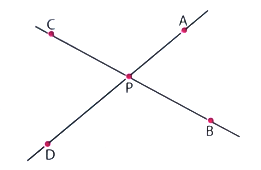
\includegraphics[width=0.5\linewidth]{6FMA69_imagens/imagem1}
		\end{center}
		Os ângulos opostos pelo vértice têm a mesma medida, ou seja:
		\begin{itemize}
			\item $A\hat{P}C$ e $B\hat{P}D$ são congruentes;
			\item $A\hat{P}B$ e $C\hat{P}D$ são congruentes.
		\end{itemize}
		Se os quatro ângulos formados forem iguais, dizemos que as retas são \textbf{perpendiculares}.
		\begin{center}
			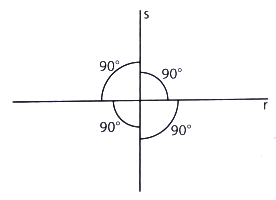
\includegraphics[width=0.5\linewidth]{6FMA69_imagens/imagem2}
		\end{center}
		Podemos representar também da seguinte forma:
		\begin{center}
			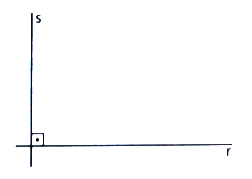
\includegraphics[width=0.5\linewidth]{6FMA69_imagens/imagem3}
		\end{center}
		\begin{itemize}
			\item Se $r~//~s$ e $s~//~t$, então $r~//~t$.
			\item Se $r~\perp~s$ e $s~\perp~t$, então $r~//~t$.
			\item Se $r~//~s$ e $s~\perp~t$, então $r~\perp~t$.
			\item Se $r~\perp~s$ e $s~//~t$, então $r~\perp~t$.
		\end{itemize}
		\noindent\textsubscript{-----------------------------------------------------------------------------------------------------------------------------------------------------------}
    	\begin{multicols}{2}
    	\begin{enumerate}
   			\item Na figura a seguir, temos duas retas que se cruzam em um ponto tal que $x = 22°$ e $z = 158°$. Dê o valor de $y$ e $w$.
   			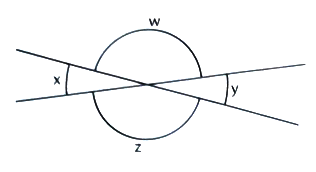
\includegraphics[width=1\linewidth]{6FMA69_imagens/imagem4} \\\\\\\\\\\\\\\\\\\\
   			\item Considere as retas $a$, $b$ e $c$, no mesmo plano, tais que $a \perp b$ e $b \perp c$. Qual é a posição entre as retas $a$ e $c$? \newpage
   			\item Dadas as retas $x$, $y$ e $z$, no mesmo plano, sabe-se que $x~//~y$ e $y \perp z$. O que se pode afirmar sobre as retas $x$ e $z$? \\\\\\\\\\\\\\\\\\\\
   			\item Num plano $\alpha$, temos as retas $p$, $q$ e $r$ tais que $p \perp q$ e $p \perp r$. Qual é a posição relativa de $q$ e $r$?\\\\\\\\\\\\\\\\\\\\
   			\item Observe o cubo a seguir e classifique as sentenças em \textbf{V} (verdadeiro) ou \textbf{F} (falso).
   			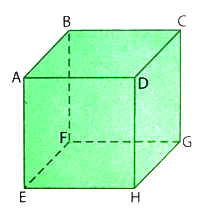
\includegraphics[width=1\linewidth]{6FMA69_imagens/imagem5} \\
   			\begin{enumerate}[a)]
   				\item (~~) $\overleftrightarrow{AB}$ e $\overleftrightarrow{EF}$ são paralelas.
   				\item (~~) $\overleftrightarrow{AE}$ e $\overleftrightarrow{GH}$ são reversas.
   				\item (~~) $\overleftrightarrow{BC}$ e $\overleftrightarrow{EH}$ são reversas.
   				\item (~~) $\overleftrightarrow{DH}$ e $\overleftrightarrow{HG}$ são perpendiculares.
   				\item (~~) $\overleftrightarrow{CD}$ e $\overleftrightarrow{EF}$ são paralelas.
   				\item (~~) $\overleftrightarrow{BC}$ e $\overleftrightarrow{CD}$ são paralelas.   				
   			\end{enumerate}
   			%75 a 78
   			\item Sejam $r_1, r_2, r_3, r_4$ retas de um mesmo plano, sendo $r_1 \cap r_2 = \varnothing$, $r_1 \perp r_3, \varnothing \neq r_2 \cap r_4 \neq r_3 \cap r_4 \neq \varnothing, r1 \cap r_4 \neq r_3 \cap r4$; considere o conjunto $S$ formado pelas intersecções das retas dadas. Quantos elementos tem $S$? \newpage
   			\item (FEI) No quadro a seguir, $a, b, c, d$ e $e$ são retas coplanares e distintas. Completando o quadro com os símbolos: \\ // ... "é paralela a" ~~~~~~~~~~~~ \\ $\perp$ ... "é perpendicular a" \\ O número total de vezes que o símbolo // aparece (incluindo o já escrito) é:
   			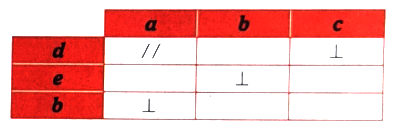
\includegraphics[width=1\linewidth]{6FMA69_imagens/imagem6} \\
   			\begin{enumerate}[a)]
   				\item 1
   				\item 2
   				\item 3
   				\item 4
   				\item 5
   			\end{enumerate}
   			\item A reta $u$ é paralela à reta $t$; a reta $t$ e a reta $v$ são concorrentes. As três retas estão no mesmo plano. O que você pode afirmar a respeito das retas $u$ e $v$? \\\\\\\\\\\\\\\\\\\\\\\\\\\\
   			\item Considere as retas $a, b$ e $c$. Sabe-se que existem pontos $M, N$ e $O$, distintos, tais que $a \cap b = \{M\}, a \cap c = \{N\}$ e $b \cap c = \{O\}$. \\
   			Faça um desenho mostrando essa situação.
	    \end{enumerate} 
        $~$ \\ $~$ \\ $~$ \\ $~$ \\ $~$ \\ $~$ \\ $~$ \\ $~$ \\ $~$ \\ $~$ \\ $~$ \\ $~$ \\ $~$  \\ $~$ \\ $~$ \\ $~$ \\ $~$ \\ $~$ \\ $~$ \\ $~$ \\ $~$ \\ $~$ \\ $~$ \\ $~$ \\ $~$ \\ $~$ \\ $~$ \\ $~$ \\ $~$ \\ $~$ \\ $~$
	\end{multicols}
\end{document}